\clearpage

\section{Ascii To Binary}

\begin{tcolorbox}	
	\begin{tabular}{p{2.75cm} p{0.2cm} p{10.5cm}} 	
		\textbf{Header File}   &:& ascii\_to\_binary\_*.h \\
		\textbf{Source File}   &:& ascii\_to\_binary\_*.cpp \\
        \textbf{Version}       &:& 20180905 (Andr\'e Mourato)
	\end{tabular}
\end{tcolorbox}

\subsection*{Methods}

AsciiToBinary(vector$\langle$Signal *$\rangle$ \&InputSig, vector$\langle$Signal *$\rangle$ \&OutputSig) :Block(InputSig, OutputSig)\{\};
\bigbreak
void initialize(void);
\bigbreak
bool runBlock(void);
\bigbreak

\subsection*{Functional description}

Figure \ref{AsciiSignalImage} shows an example of an input signal that can be passed as argument. This signal contains three characters: a, b and c. Each character can be represented by 8 bits, according to the Ascii Table. The values to these three characters are respectively: $01100001$, $1100010$ and $1100011$.
The block AsciiToBinary will convert the characters a, b and c to their respective binary codes. The resulting output signal will be of type Binary. The output signal to this example, shown in figure \ref{BinarySignalImage}, is the concatenation of the previous binary codes. The full binary sequence is $0110000111000101100011$.

\begin{figure}[h]
	\centering
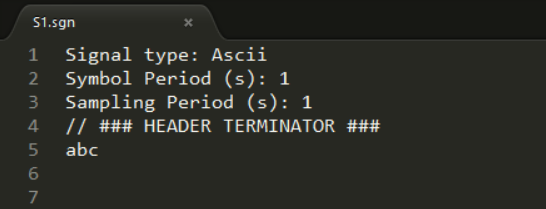
\includegraphics[width=.7\linewidth]{./lib/ascii_to_binary/figures/ascii_signal.png}
\caption{Ascii signal passed as input to the AsciiToBinary block}\label{AsciiSignalImage}
\end{figure}

\begin{figure}[h]
	\centering
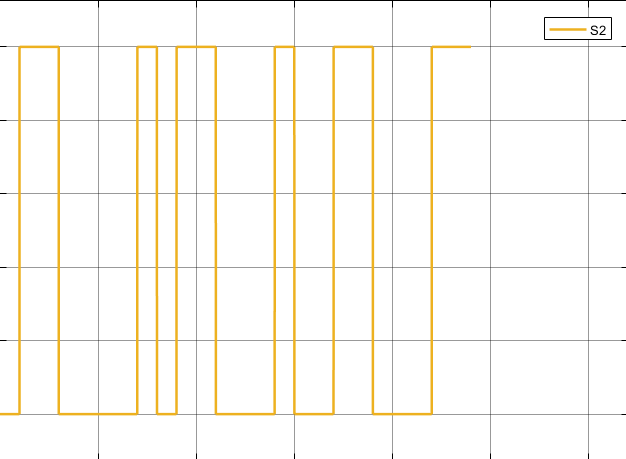
\includegraphics[width=.5\linewidth]{./lib/ascii_to_binary/figures/binary_signal.png}
\caption{Resulting Binary signal from the output of the AsciiToBinary block}\label{BinarySignalImage}
\end{figure}
\pagebreak

\subsection*{Input Signals}

\subparagraph*{Number:} 1

\subparagraph*{Type:} Ascii

\subsection*{Output Signals}

\subparagraph*{Number:} 1

\subparagraph*{Type:} Ascii